\documentclass[conference]{IEEEtran}
\IEEEoverridecommandlockouts
% The preceding line is only needed to identify funding in the first footnote. If that is unneeded, please comment it out.
\usepackage{cite}
\usepackage{amsmath,amssymb,amsfonts}
\usepackage{algorithmic}
\usepackage{graphicx}
\usepackage{textcomp}
\usepackage{xcolor}
\def\BibTeX{{\rm B\kern-.05em{\sc i\kern-.025em b}\kern-.08em
    T\kern-.1667em\lower.7ex\hbox{E}\kern-.125emX}}
\begin{document}

\title{Self-Cleaning Transmitters in Diffusion-based Molecular Communcation\\
}

\author{\IEEEauthorblockN{Ethan Fox}
\IEEEauthorblockA{\textit{Undergraduate Student} \\
\textit{University of Nebraska-Lincoln}\\
Lincoln, NE USA \\
efox@huskers.unl.edu}
\and
\IEEEauthorblockN{Jackson Herman}
\IEEEauthorblockA{\textit{Undergraduate Student} \\
\textit{University of Nebraska-Lincoln}\\
Lincoln, NE USA \\
jherman5@huskers.unl.edu}
}

\maketitle

\begin{abstract}
This document is a model and instructions for \LaTeX.
This and the IEEEtran.cls file define the components of your paper [title, text, heads, etc.]. *CRITICAL: Do Not Use Symbols, Special Characters, Footnotes, 
or Math in Paper Title or Abstract.
\end{abstract}

\begin{IEEEkeywords}
component, formatting, style, styling, insert
\end{IEEEkeywords}

\section{Introduction}
This document is a model and instructions for \LaTeX.
Please observe the conference page limits. 

\subsection{Background}

The concept of using molecules and biological processes to emulate traditional computer communication networks is a relatively new field of research, and as such there are plenty of areas within it where new advancements and discoveries can be made. For example, in a diffusion-based communication system one of the most prevalent problems is the channel being clogged by transmitted molecules, leading to inaccurate data as the receiver detects molecules, even when it shouldn’t be.
\\
\par
Efforts have been made to find ways to clear the channel, one such method is the concept of releasing an additional molecule into the channel whose sole purpose is to break down any remaining transmitted molecule to prevent the receiver incorrectly reading a transmitted bit when there isn’t supposed to be one. However, this method suffers a similar problem to not clearing the channel at all, except now instead of the transmitted molecules it is the clearing ones that remain, meaning any molecules sent to transmit a new bit could be broken down before they can reach the receiver, leading to a false negative as opposed to the false positives that not clearing can cause. These problems, caused by the channel being clogged by leftover molecules, is what the experiment detailed in this report endeavors to solve.

\section{Design}

\subsection{Logic Gate Design}
Before delving into solving the problems with channel clearing and saturation, first a communication system is needed to perform tests on. This experiment utilizes a simple system of a single receiver and two transmitters placed at equal distances horizontally from the receiver and at equal and opposite vertical distances.

\begin{figure}
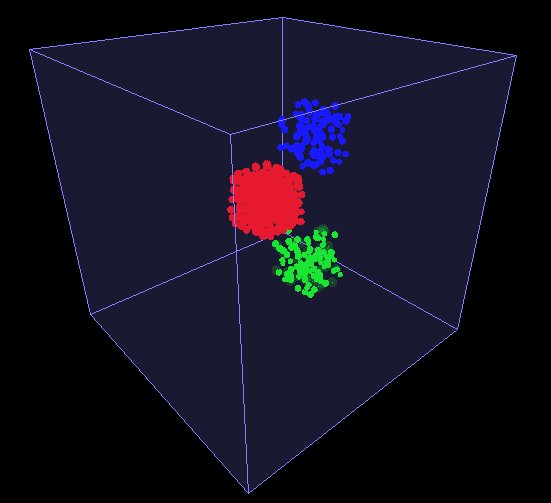
\includegraphics[width=\linewidth]{System.png}
\caption{Fig 1: Receiver represented in red, transmitters represented in blue and green.}
\end{figure}

The experiment was performed utilizing the Simulation tool BSim \cite{b1}, and was done in a large 3-Dimensional space as to most accurately represent the environment a real form of the experiment would occur within the human body.
\\
\par
The sizes of all three bacteria populations remained constant throughout the main portion of the experiment, as well as the molecule vesiculation rate and the time the molecules have to propagate towards the receiver before the output is computed, more about these constants will be discussed in the Experiment Design section of this report. The system was built to act as either a simple AND logic gate or a simple OR logic gate, and the output of the receiver changed to reflect its behavior.

\subsection{Clearing Design}

After the transmitter molecules have been given enough time to propagate through the channel, the clearing process begins. The two transmitters cooperate together towards the end of every time slot to clear the channel of any extra transmitter molecules. Both populations start to produce clearing molecules that propagate after the transmitter molecules, and upon contact with a transmitter molecule, they neutralize it, preventing it from binding to the receiver.
\\
\par
To achieve this neutralization, a hypothetical molecule is used that will bind with a transmitter molecule, preventing it from binding with anything else, be it the receiver or another clearing molecule. Each clearing molecule will similarly only be able to bind with a single transmitter molecule. Thus, a collision between the two molecules would effectively neutralize them both, preventing the transmitter molecule from causing false positives, and the clearing molecule from causing false positives.

\begin{figure}
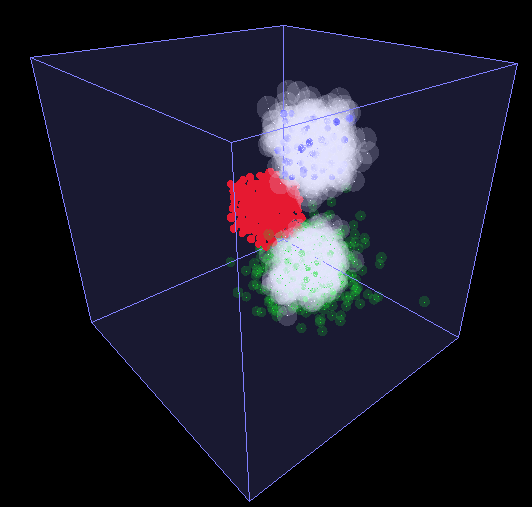
\includegraphics[width=\linewidth]{Clearing.png}
\caption{Fig 2: Populations A and B producing clearing molecules, represented in white.}
\end{figure}

\section{Experiment Design}

The core premise of this experiment is to find out how the cooperation of the transmitters to clear the channel, as well as the neutralization method of clearing, affect the accuracy and reliability of the system when compared to a system with no clearing.

\subsection{Finding a Control Test}

To be able to effectively test the change in accuracy and reliability, a set of control constants needed to be found for the system. The criteria the control test needed to meet was to be able to detect both a 1 bit within a specific time slot both when sent as the first bit of the bitstring, as well as when sent after nothing has been sent for a time slot to represent the bit sequence 01. First, a suitable distance was set for the channel between the transmitters and receivers. These values were not tweaked during the testing of other values when searching for an optimal control test. The center of each transmitter population was set to 20 microns along the x-axis away from the center of the receiver, 20 microns away along the y-axis, and 5 microns away along the z-axis. 
\\
\par
The values of the control that were tested were all changed with respect to these distances. Of these values, the one that was tweaked first was the time slot duration. This is how long the receiver will detect collisions from transmitter molecules before determining the output. In each test, the transmitter would only generate molecules for half the time slot, to reduce channel clutter. This buffer period was kept in tests beyond the search for the control. For the duration of these tests, the transmitter population sizes were 100 each, the receivers population size was 250, and the threshold of collisions detected for a 1 to be outputted was set to 100. With these tests, a bit string of size three was sent from each transmitter, 100 from transmitter A, and 010 from transmitter B.

\begin{table}[htbp]
\begin{center}
\begin{tabular}{|c|c|c|c|c|}
\hline
Time Slot & Sent A & Sent B & Received A & Received B\\\hline
10 & 100 & 010 & 000 & 000\\\hline
20 & 100 & 010 & 110 & 000\\\hline
30 & 100 & 010 & 110 & 001\\\hline
\end{tabular}
\end{center}
\caption{Fig 3: Results from changing the time slot duration.}
\end{table}

From these tests, it was believed that 30 seconds was a suitable time slot duration, so long as other values were tweaked accordingly. Thus, the next set of values changed was the threshold. Population sizes were kept the same as the previous tests, and a 30 second time slot duration was used.

\begin{table}[htbp]
\begin{center}
\begin{tabular}{|c|c|c|c|c|}
\hline
Threshold & Sent A & Sent B & Received A & Received B\\\hline
80 & 100 & 010 & 110 & 001\\\hline
60 & 100 & 010 & 110 & 001\\\hline
40 & 100 & 010 & 111 & 011\\\hline
\end{tabular}
\end{center}
\caption{Fig 4: Results from changing the threshold.}
\end{table}

The first 1 of population B’s bit string was read correctly in the test with the threshold of 40, however that threshold was determined to be too low to get accurate results, as the first 1 from population A’s bit string was stretching to 3 time slots instead of the 2 it lasted in higher thresholds. Thus, the threshold was returned to 100, and a 40 second time slot was tested. This test resulted in a 110 from A and a 011 from B, which were satisfactory results. With that, the constant had been decided, and the control test accomplished. Now, testing could be done to compare clearing against the control.

\subsection{Comparing No Clearing and Clearing}

Now that a control test has been set, it can be used for tests without clearing to be compared against tests with clearing. When introducing the clearing molecules to the channel, a buffer period is present, similar to the control test, however part way through that buffer is when the clearing molecules are generated into the channel.
\\
\par
Each transmitter generates its transmission molecules for 50\% of the time slot duration, and then the next 25\% is a buffer period to allow it to propagate, and then the last 25\% is when the clearing molecules are generated. With these clearing molecules generated, hopefully the channel will be less saturated, and less false positives and negatives are read.


\section{Simulation Results}

\section{Conclusion}

\begin{thebibliography}{00}
\bibitem{b1} Matyjaszkiewicz A, Fiore G, et al. (2017) BSim 2.0: An Advanced Agent-Based Cell Simulator. ACS Synthetic Biology (web)Article ASAP doi:10.1021/acssynbio.7b00121
\vspace{12pt}
\color{red}
\end{thebibliography}
\end{document}